\documentclass[12pt]{article}

\usepackage{graphicx}
\usepackage{float}
\usepackage[margin=1in]{geometry}
\usepackage{longtable}
\usepackage{setspace}

\title{Dog Shelter Management System\\Design Specification}
\author{
Fernando Camberos \\
Kwane Galang \\
Korapat Jaengsrivong \\
Andy Lim \\
Fredy Lung
}
\date{May 2026}

\begin{document}

\maketitle

\tableofcontents
\newpage

\section*{Revision History}
\begin{longtable}{|c|p{5cm}|c|c|c|}
\hline
\textbf{Revision \#} & \textbf{Change Description} & \textbf{Date} & \textbf{Revised By} & \textbf{Approved By} \\
\hline
1.0 & Initial Design Specification including core pages and features & 05/06/2026 & & \\
\hline
1.1 & Added Dog Intake and Status Tracking pages and interactions & 05/07/2026 & & \\
\hline
1.2 & Added Medical Records, Adoption System, and Dashboard pages & 05/08/2026 & & \\
\hline
1.3 & Final refinements and future work additions & 05/09/2026 & & \\
\hline
\end{longtable}

\newpage

\section{Introduction}

\subsection{Purpose}
This Design Specification document describes the structure and layout of the Dog Shelter Management System. It provides a detailed breakdown of system pages, features, and user interactions.

\subsection{Intended Audience}
This document is intended for developers, project managers, and stakeholders who need a clear understanding of the system layout and functionality.

\subsection{System Overview}
The system is a web-based application designed to manage shelter operations including dog intake, medical tracking, adoption processing, and status management. It supports both public users and staff users.

\subsection{Scope}
This document defines the system’s user interface structure and feature breakdown. It complements the SRS and SDD by focusing on how features are presented and used within the system.

\section{System Overview and Navigation}

The system consists of multiple pages accessible based on user roles:

\begin{itemize}
\item Public Users: Can view dogs and submit adoption applications
\item Staff/Admin: Can manage dogs, medical records, and applications
\end{itemize}

Navigation is handled through a web-based interface where users interact with pages that communicate with the backend API and database.

\section{Page and Feature Breakdown}

\subsection{Home / Dog Listing Page}
Displays all dogs with their current status (Available, Pending, Adopted).

\textbf{Features:}
\begin{itemize}
\item View list of dogs
\item Filter by status
\item Search dogs
\item Navigate to Dog Profile
\end{itemize}

\begin{figure}[H]
    \centering
    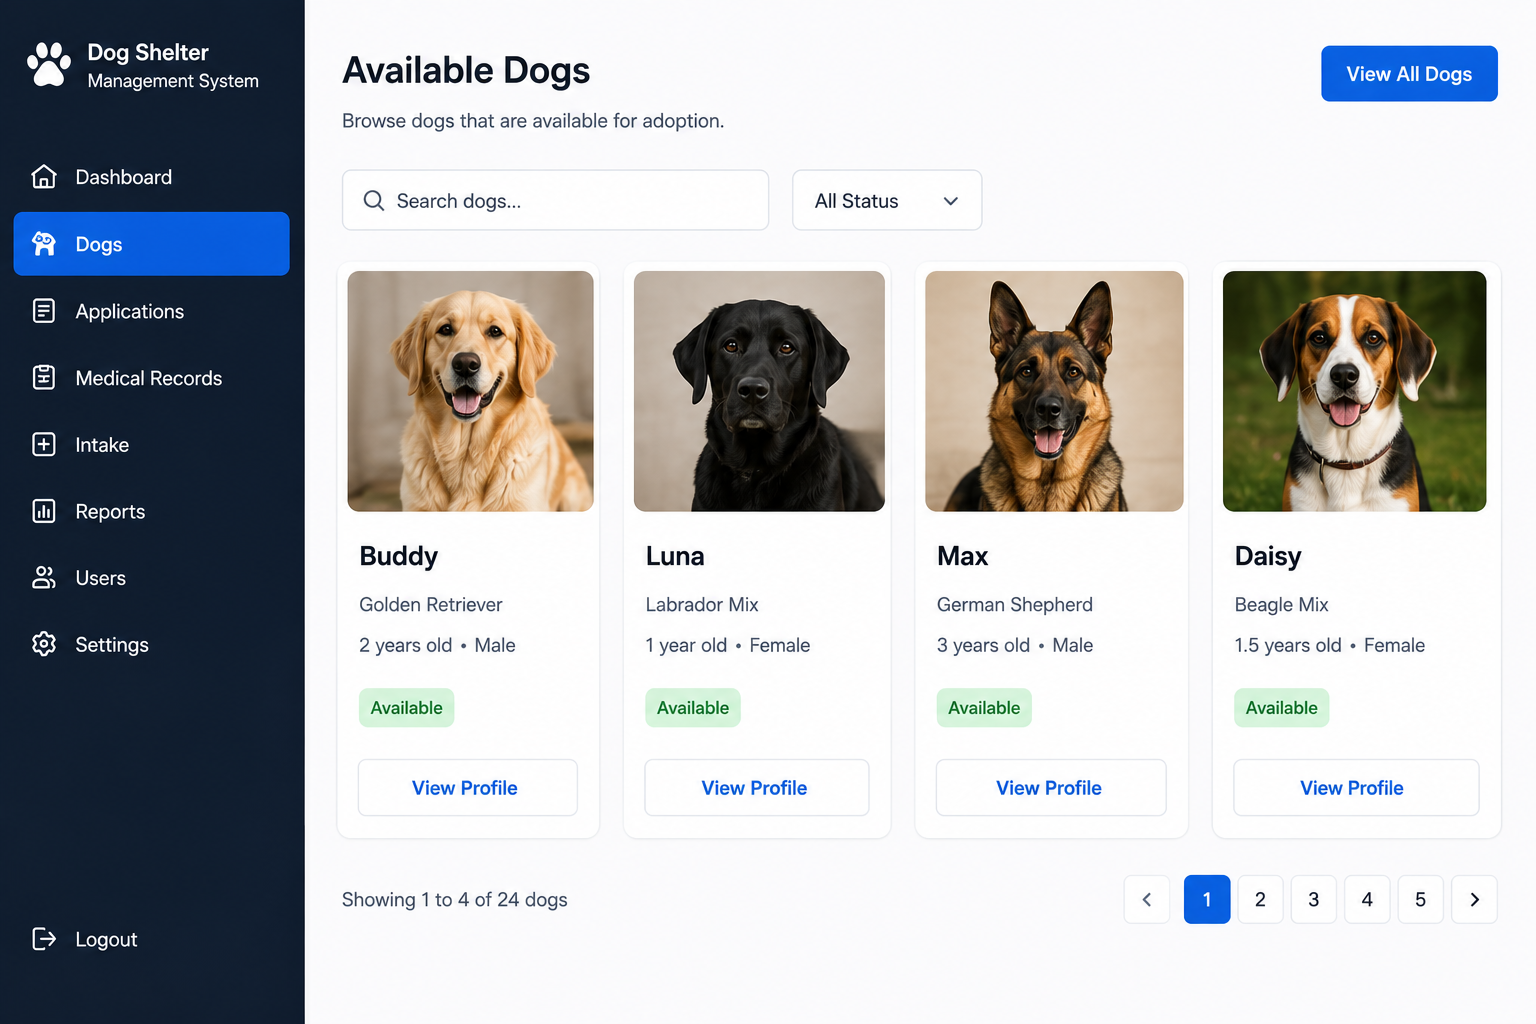
\includegraphics[width=0.9\textwidth]{images/dog_listing.png}
    \caption{Dog Listing Page displaying available dogs with filtering and search functionality.}
    \label{fig:dog_listing}
\end{figure}


\subsection{Dog Profile Page}
Displays detailed information for a selected dog.

\textbf{Features:}
\begin{itemize}
\item View dog information (name, breed, age)
\item View current status
\item View medical records
\item View adoption applications (staff only)
\end{itemize}

\begin{figure}[H]
    \centering
    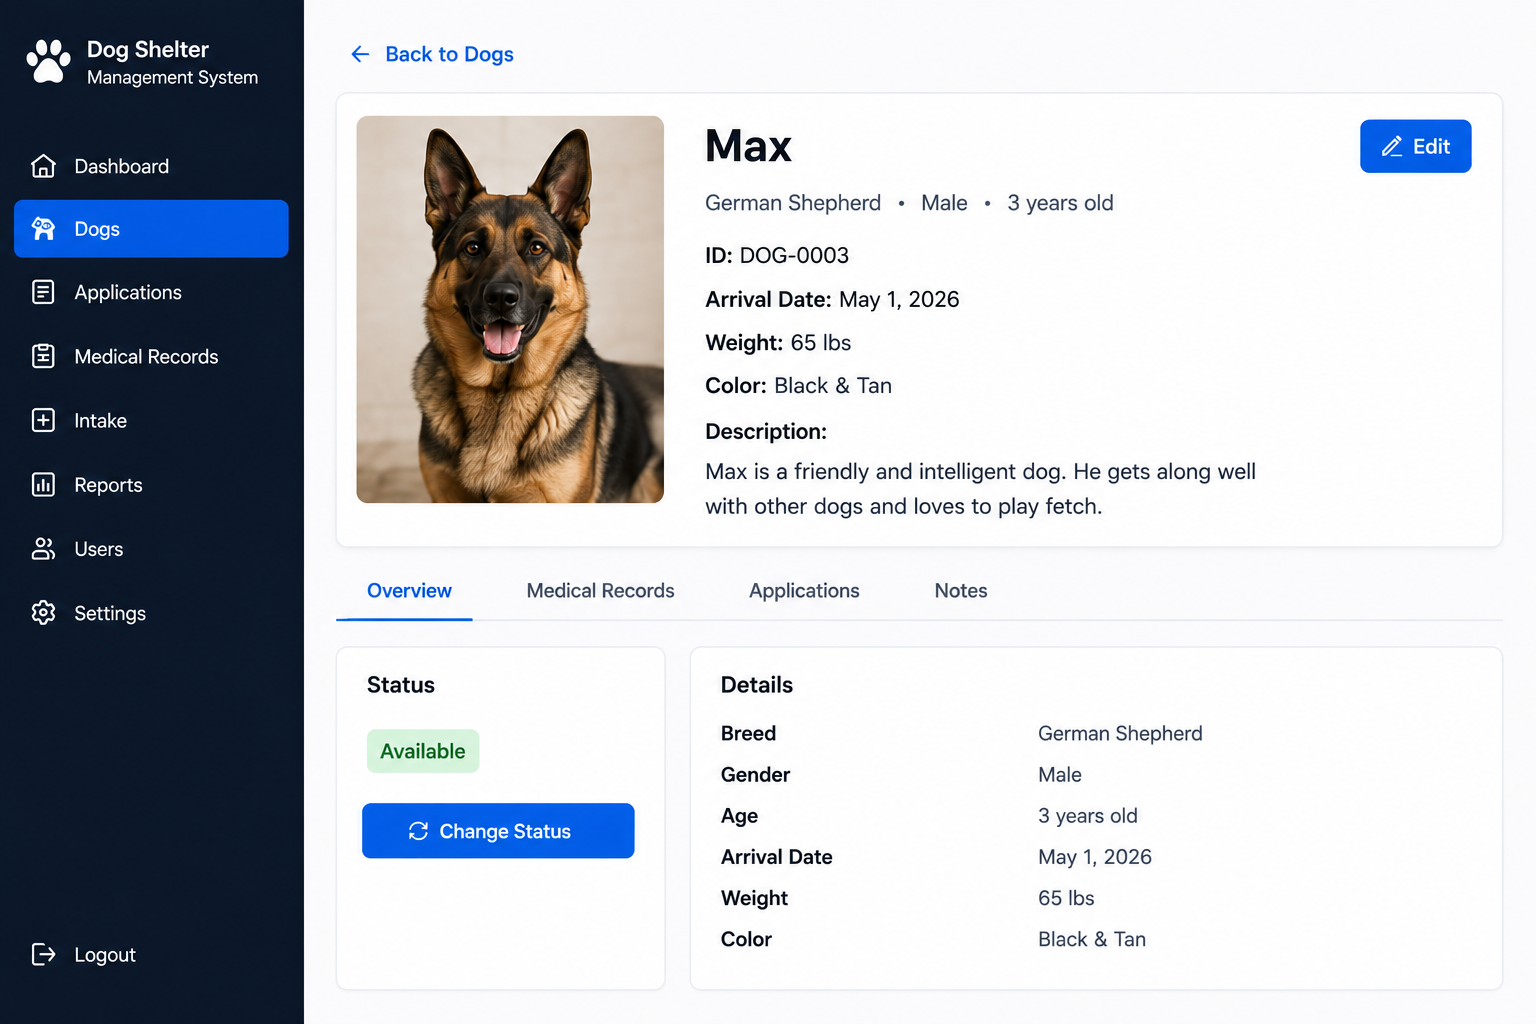
\includegraphics[width=0.9\textwidth]{images/dog_profile.png}
    \caption{Dog Profile Page showing detailed information, status, and related records for a selected dog.}
    \label{fig:dog_profile}
\end{figure}

\subsection{Dog Intake Page}
Allows staff to add new dogs to the system.

\textbf{Inputs:}
\begin{itemize}
\item Name, Breed, Age, Sex
\item Arrival Date
\item Intake Notes
\item Initial Status
\end{itemize}

\textbf{Behavior:}
\begin{itemize}
\item Creates a new dog record
\item Stores data in the database
\item Displays dog in listing page
\end{itemize}

\begin{figure}[H]
    \centering
    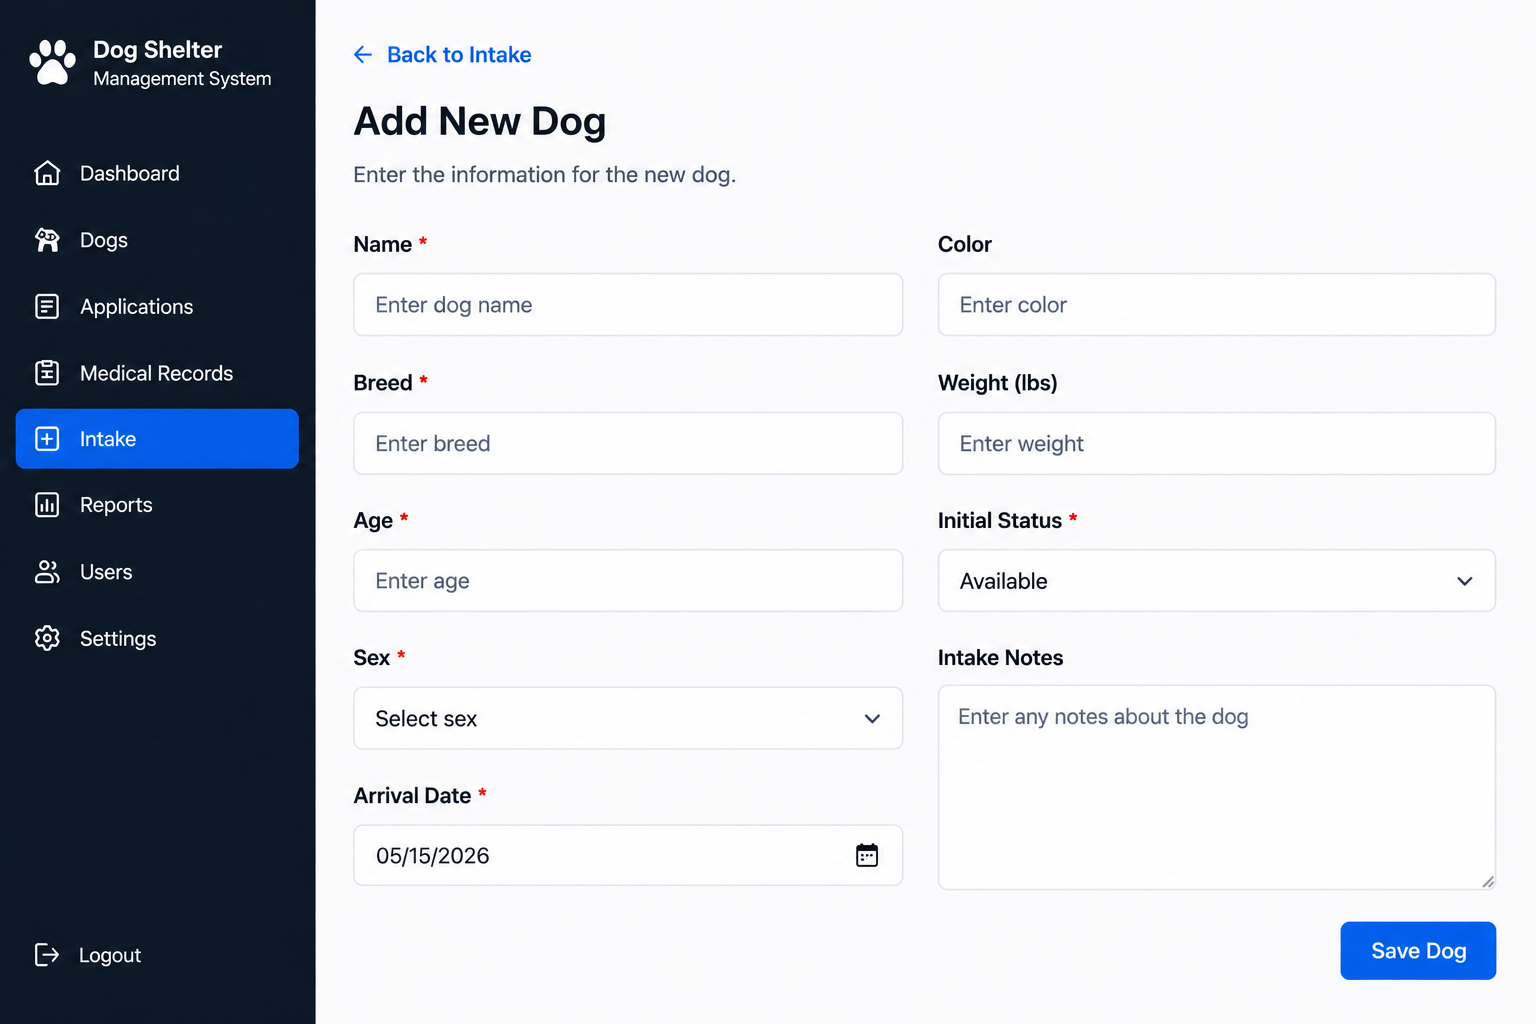
\includegraphics[width=0.9\textwidth]{images/dog_intake.png}
    \caption{Dog Intake Page allowing staff to enter and store new dog information.}
    \label{fig:dog_intake}
\end{figure}

\subsection{Dog Status Tracking}
Tracks and updates dog availability.

\textbf{Statuses:}
\begin{itemize}
\item Available
\item Pending
\item Adopted
\end{itemize}

\textbf{Behavior:}
\begin{itemize}
\item Updated by staff or system actions
\item Controls visibility on public pages
\end{itemize}

\subsection{Medical Records Page}
Allows staff to manage health data for dogs.

\textbf{Features:}
\begin{itemize}
\item Add vaccination records
\item Update health status
\item View medical history
\end{itemize}

\begin{figure}[H]
    \centering
    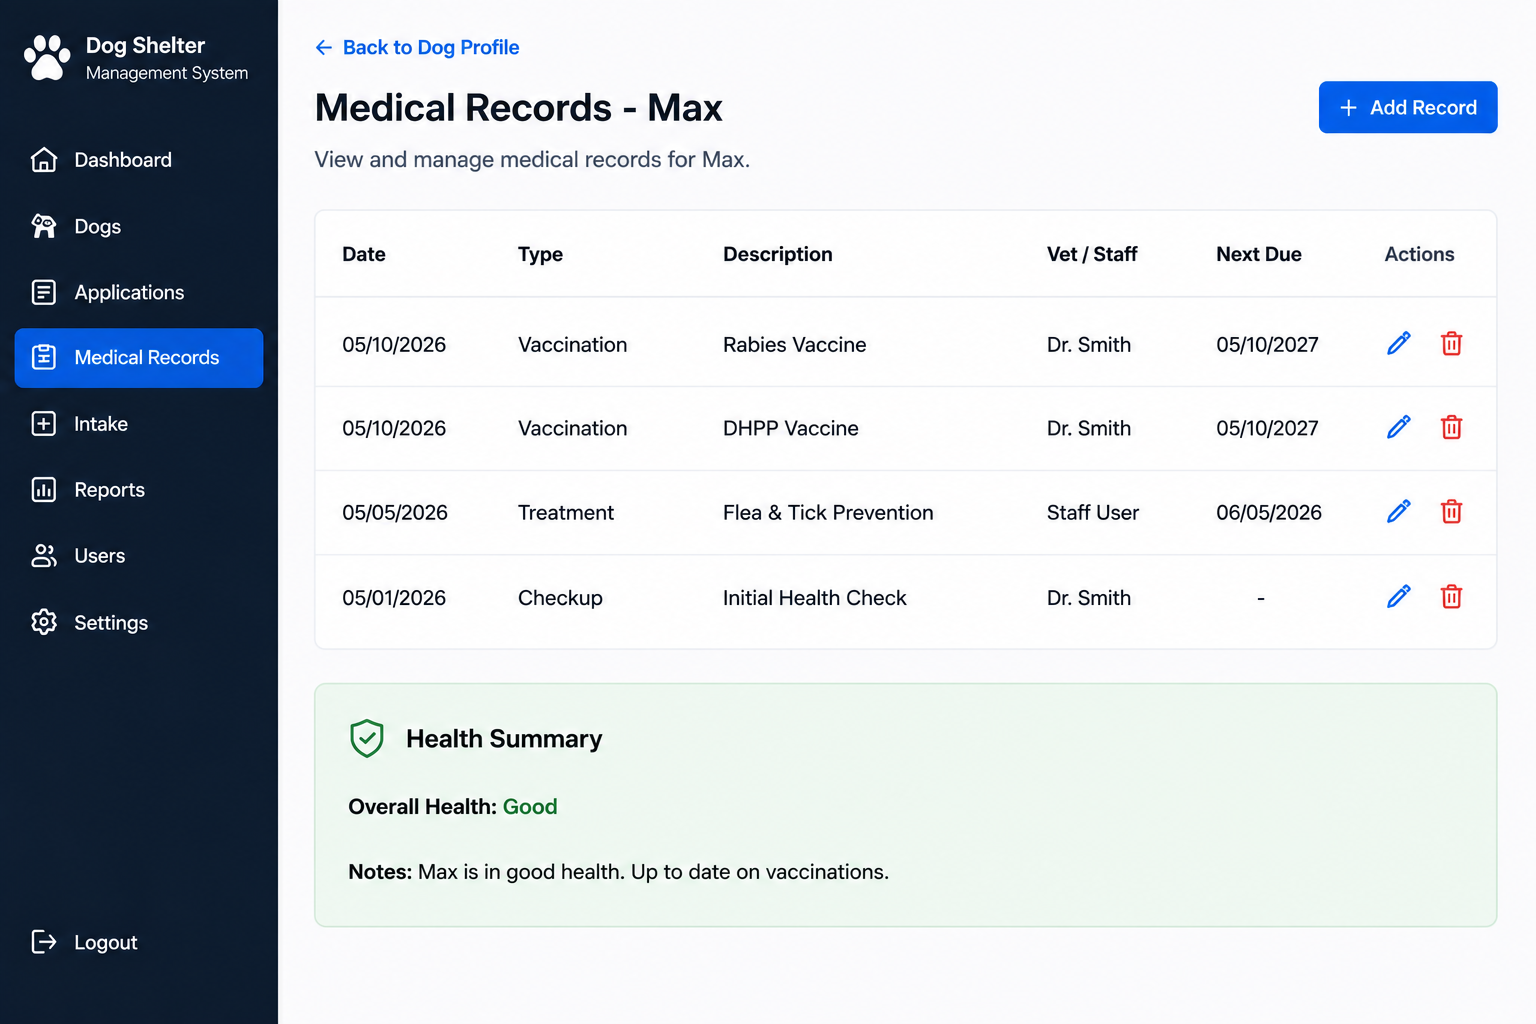
\includegraphics[width=0.9\textwidth]{images/medical_records.png}
    \caption{Medical Records Page displaying vaccination history, treatments, and health status updates.}
    \label{fig:medical_records}
\end{figure}

\subsection{Adoption Application Page}
Allows users to submit applications.

\textbf{Inputs:}
\begin{itemize}
\item Applicant name
\item Contact information
\item Address
\item Pet experience
\item Selected dog
\end{itemize}

\textbf{Behavior:}
\begin{itemize}
\item Stores application in database
\item Sets status to Pending
\end{itemize}

\begin{figure}[H]
    \centering
    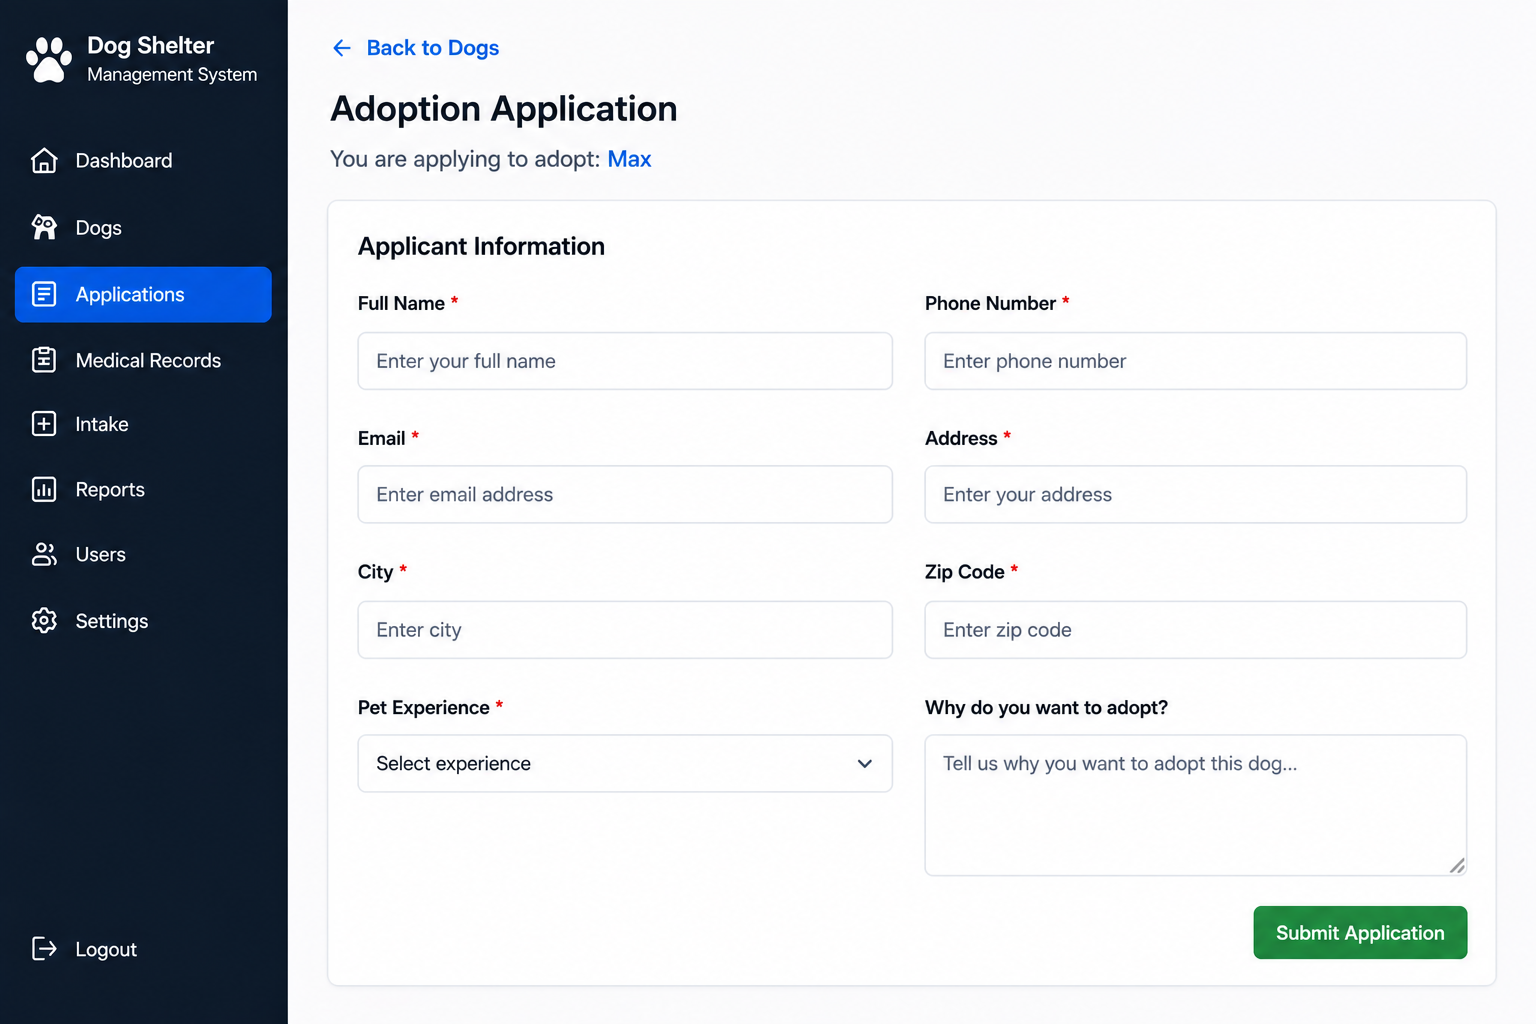
\includegraphics[width=0.9\textwidth]{images/adoption_application.png}
    \caption{Adoption Application Page where users submit requests to adopt a dog.}
    \label{fig:adoption_application}
\end{figure}

\subsection{Application Review Page}
Allows staff to review applications.

\textbf{Actions:}
\begin{itemize}
\item Approve application
\item Reject application
\item Add notes
\end{itemize}

\textbf{Behavior:}
\begin{itemize}
\item Updates application status
\item Updates dog status accordingly
\end{itemize}

\begin{figure}[H]
    \centering
    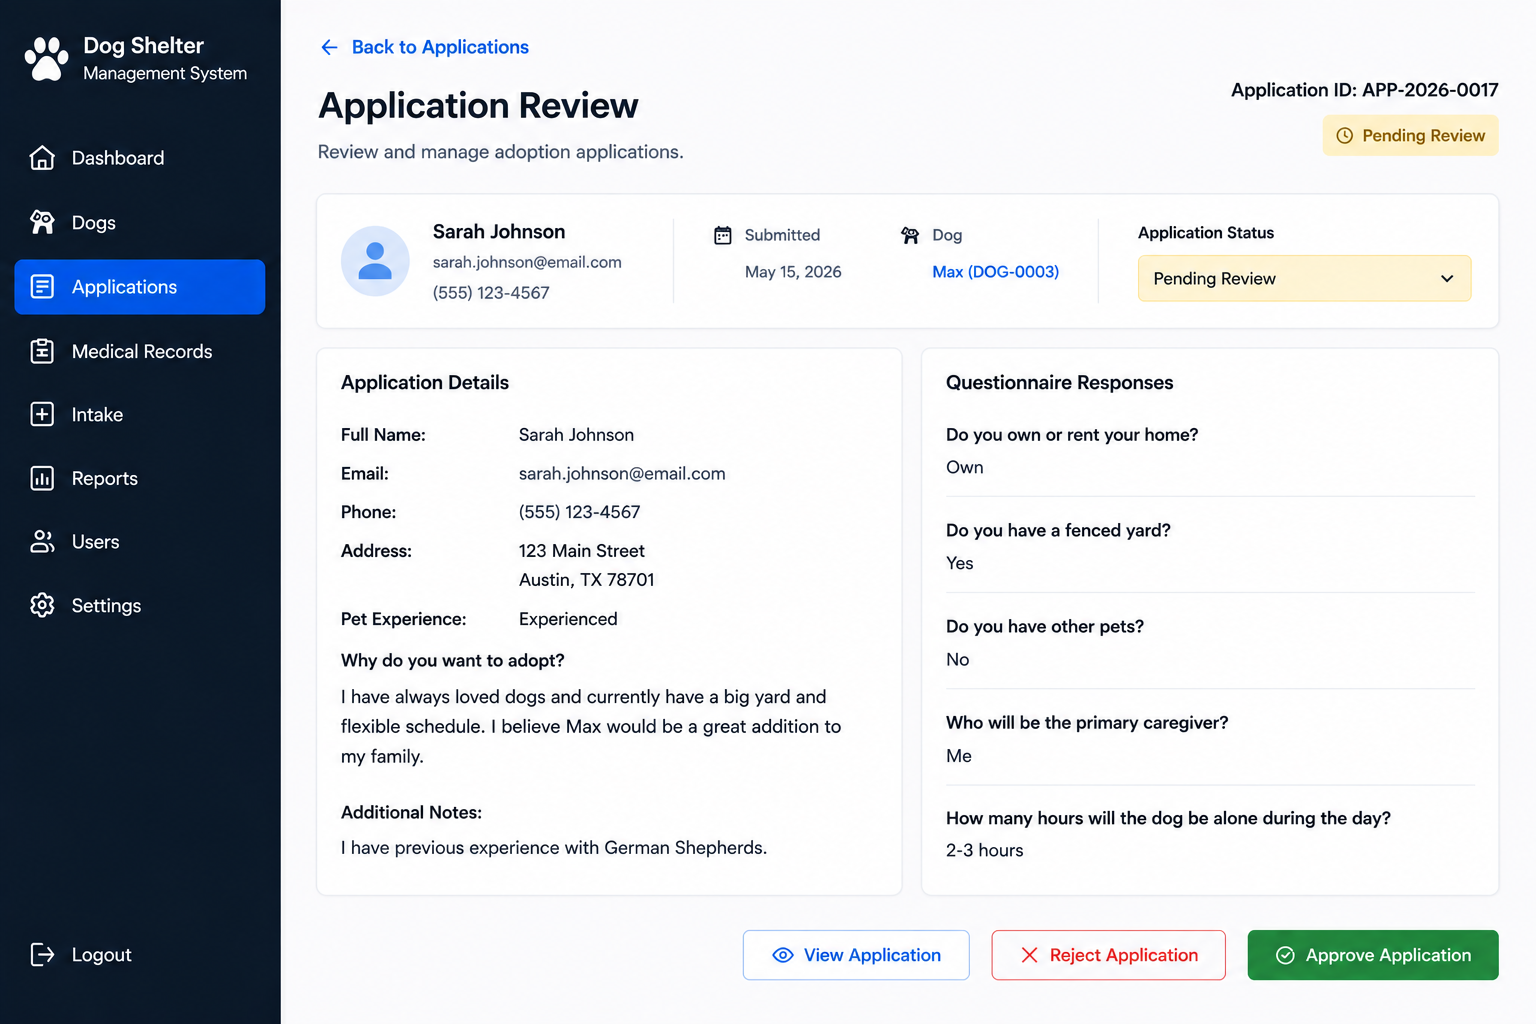
\includegraphics[width=0.9\textwidth]{images/application_review.png}
    \caption{Application Review Page allowing staff to evaluate and manage adoption applications.}
    \label{fig:application_review}
\end{figure}

\subsection{Admin Dashboard}
Central management page for staff.

\textbf{Features:}
\begin{itemize}
\item View total dogs
\item View dogs by status
\item View pending applications
\item Manage system data
\end{itemize}

\begin{figure}[H]
    \centering
    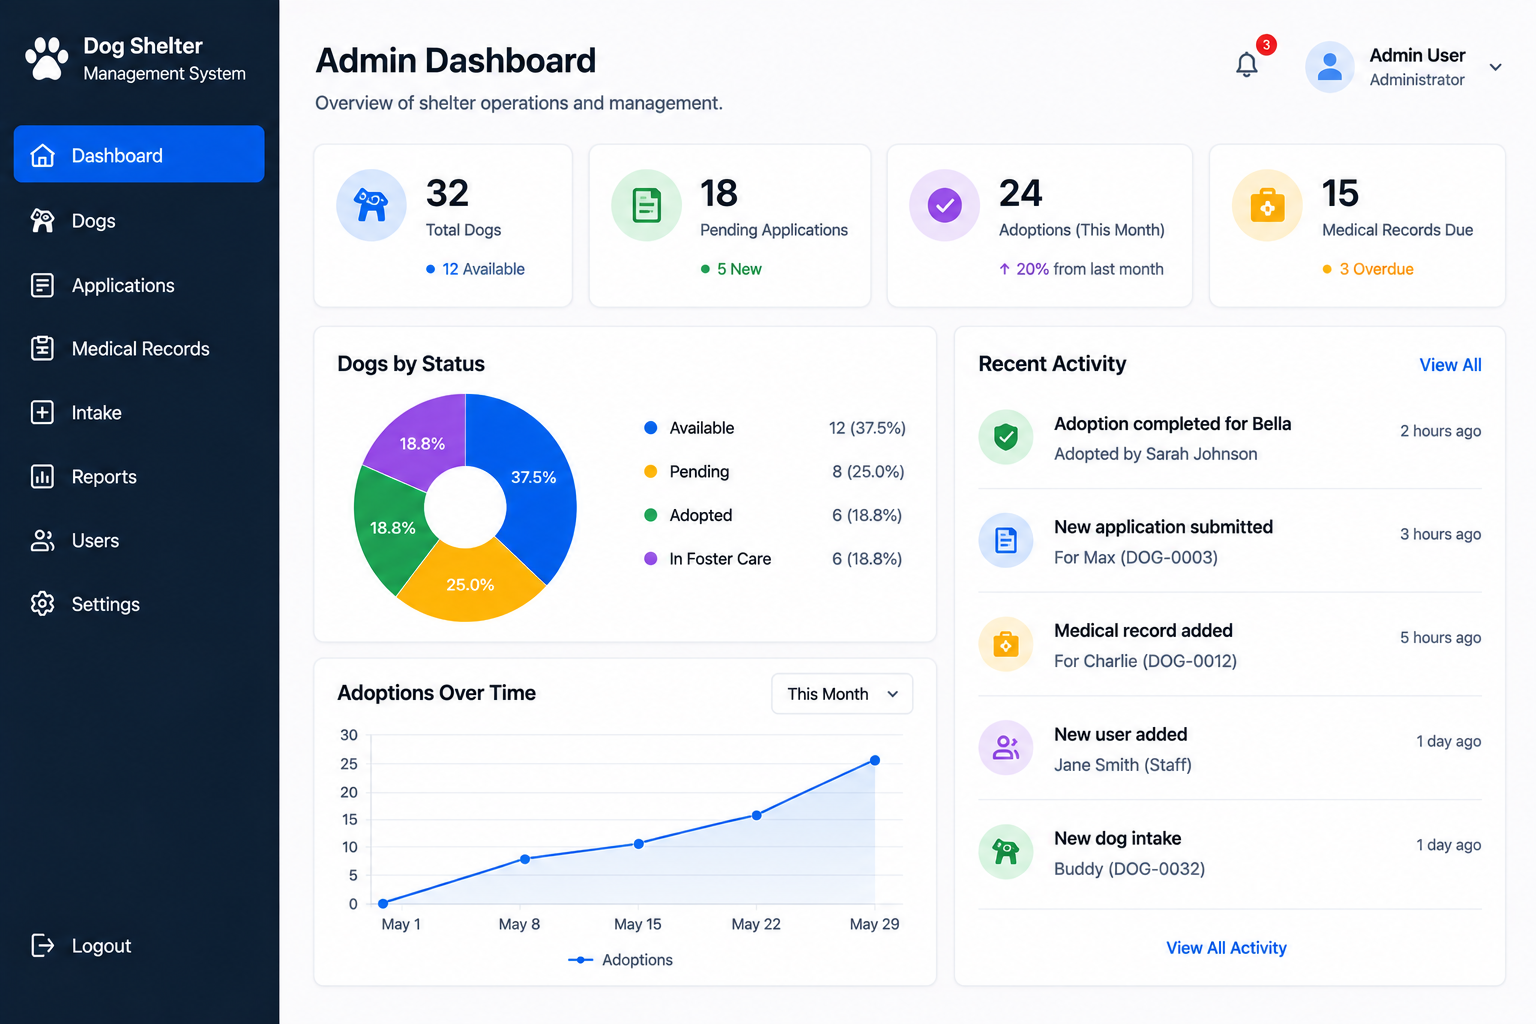
\includegraphics[width=0.9\textwidth]{images/admin_dashboard.png}
    \caption{Admin Dashboard providing an overview of system data, including dog counts, applications, and activity.}
    \label{fig:admin_dashboard}
\end{figure}

\section{Workflow Overview}

The system follows a standard interaction flow:

\begin{enumerate}
\item Staff adds a dog using the Dog Intake Page
\item Dog is stored in the database and appears as Available
\item Users view dogs and submit adoption applications
\item Staff reviews applications
\item Approved applications change dog status to Pending
\item Final adoption updates status to Adopted
\item Dashboard reflects all updates
\end{enumerate}

\section{Workflow Diagram}

\begin{figure}[H]
    \centering
    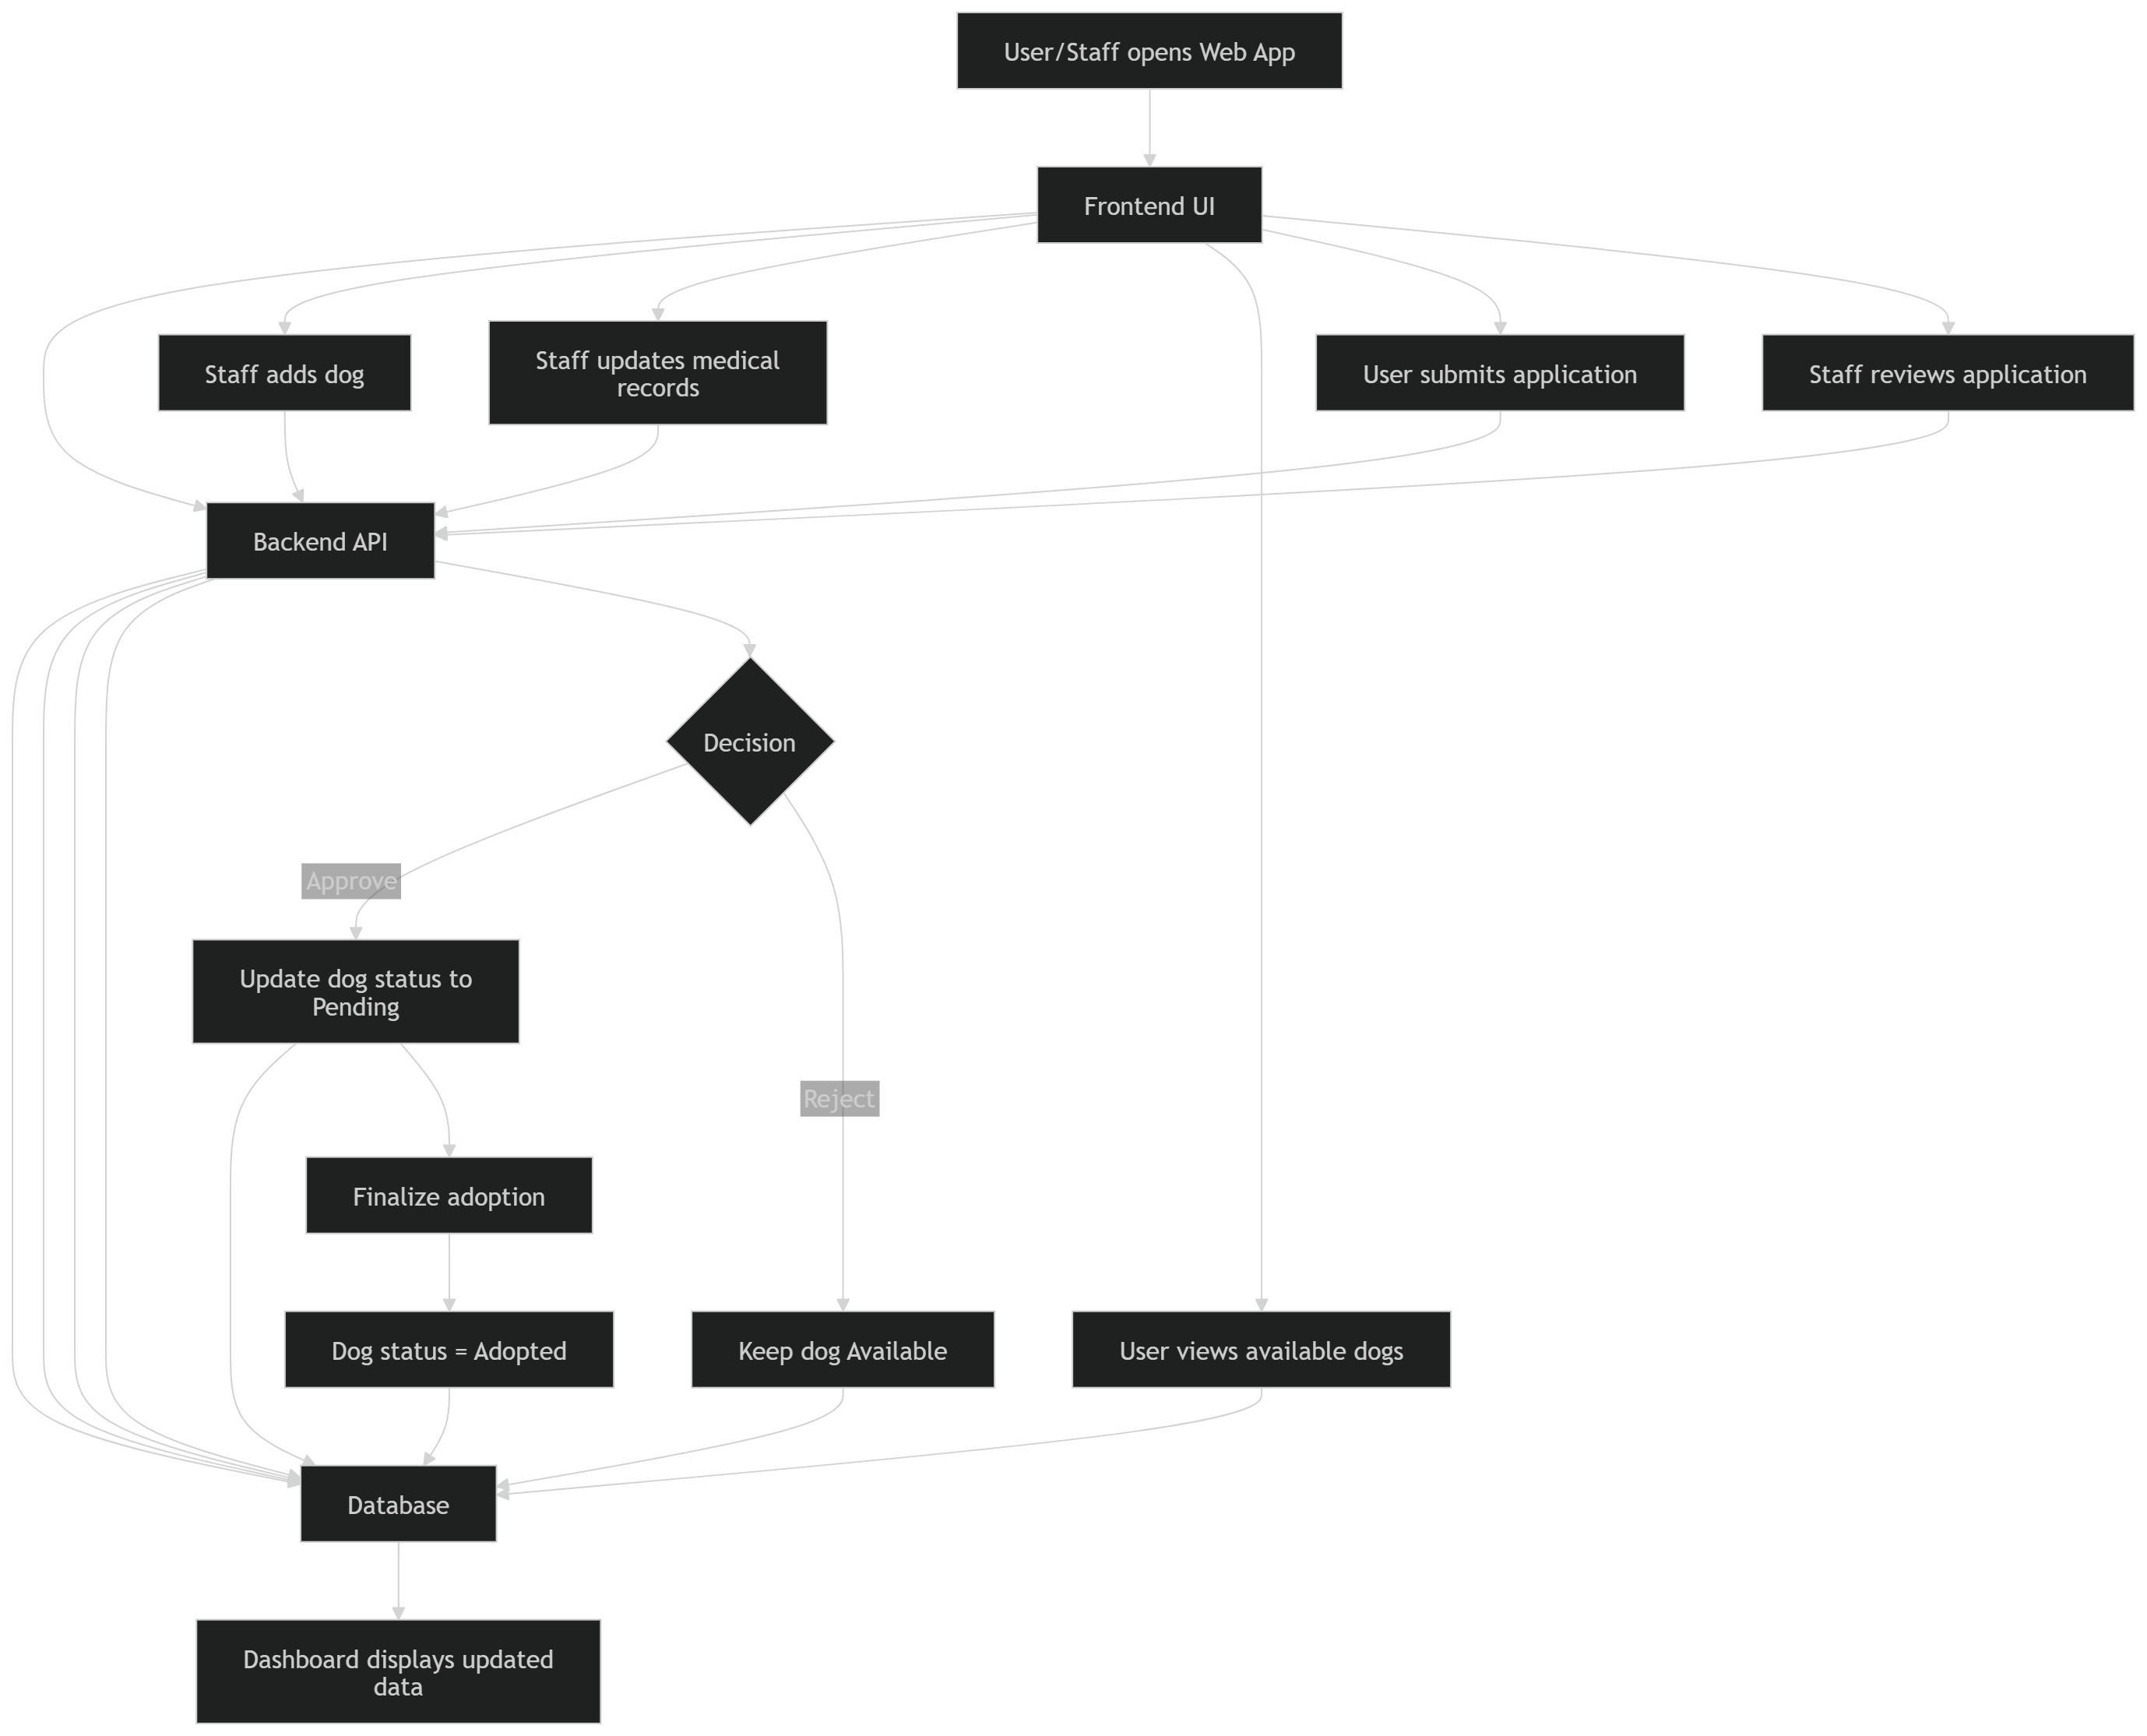
\includegraphics[width=0.8\textwidth]{images/workflow.png}
    \caption{High-level workflow diagram of the Dog Shelter Management System showing interaction between users, frontend, backend API, and database.}
    \label{fig:workflow}
\end{figure}

As shown in Figure~\ref{fig:workflow}, the system processes user and staff interactions through a web-based frontend interface. Requests are sent to the backend API, which handles business logic and communicates with the database to store and retrieve information. The workflow ensures that dog intake, medical updates, and adoption processes are consistently managed across the system.

\section{System Dependencies and Technologies}

The Dog Shelter Management System relies on the following technologies and dependencies to function within a Dockerized environment.

\subsection{Frontend}
\begin{itemize}
\item React.js
\item react-dom
\item react-scripts
\item Axios (API communication)
\item Bootstrap or Material UI (UI components)
\end{itemize}

\subsection{Backend}
\begin{itemize}
\item Node.js
\item Express.js
\item body-parser
\item cors
\item dotenv
\item jsonwebtoken (authentication)
\end{itemize}

\subsection{Database}
\begin{itemize}
\item MySQL
\item mysql2 (Node.js connector)
\end{itemize}

\subsection{Development Tools}
\begin{itemize}
\item Docker
\item Docker Compose
\item GitHub (version control)
\end{itemize}

\section{Future Work}

Potential future enhancements include:

\begin{itemize}
\item Email notifications for application status
\item Image uploads for dog profiles
\item Advanced search and filtering
\item Appointment scheduling for adoption visits
\end{itemize}

\section{Glossary}

\begin{longtable}{|c|p{8cm}|}
\hline
\textbf{Term} & \textbf{Definition} \\
\hline
Intake & Process of adding a new dog \\
\hline
Status & Current state of a dog (Available, Pending, Adopted) \\
\hline
Application & Request submitted by a user to adopt a dog \\
\hline
Dashboard & Admin interface for managing system data \\
\hline
\end{longtable}

\section{References}

\begin{itemize}
\item SRS Document
\item SDD Document
\item CS3338 Project Guidelines
\end{itemize}

\end{document}